\section {Appendix}
\subsection{Logistic Regression on Behavior Data}

\begin{figure}[H] 
\centering 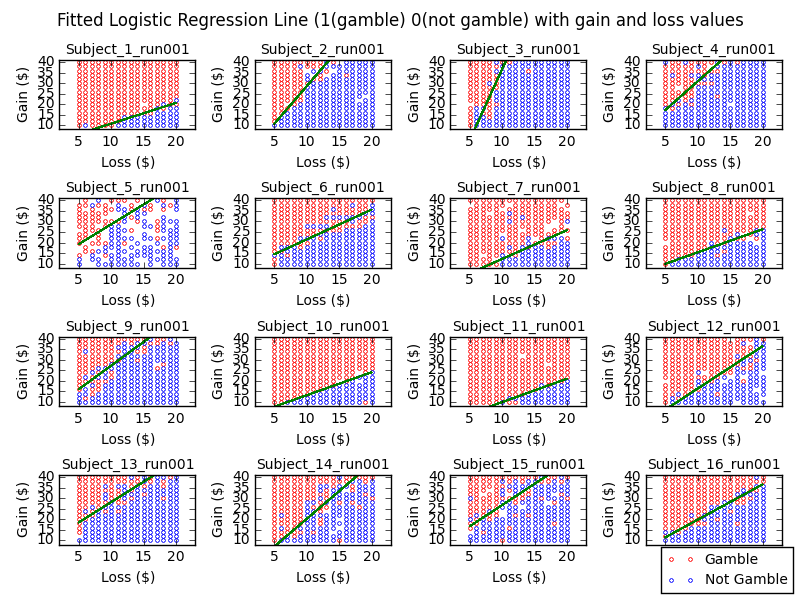
\includegraphics[scale=0.5]{../fig/log_reg_behav/log_regression_behav_subplots.png}	 
\caption{Logistic Regression on each subjects’ behavior data}
\end{figure} 

\subsection{Multi-comparison across 16 subjects on TASK condition}
\begin{figure}[H] 
\centering 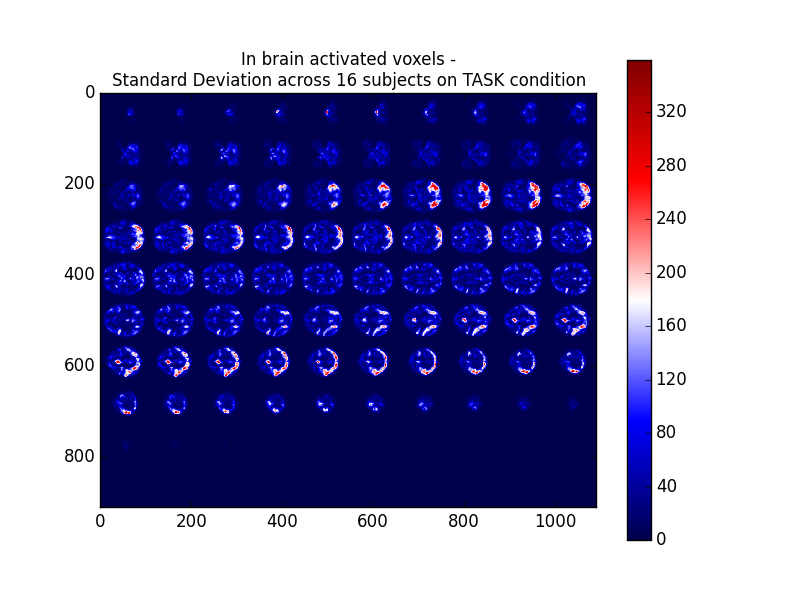
\includegraphics[scale=0.5]{../fig/multi_beta/std_task.png}	 
\caption{Standard Deviation of beta values on each voxel across 16 subjects on TASK condition}
\end{figure} 

\begin{figure}[H] 
\centering 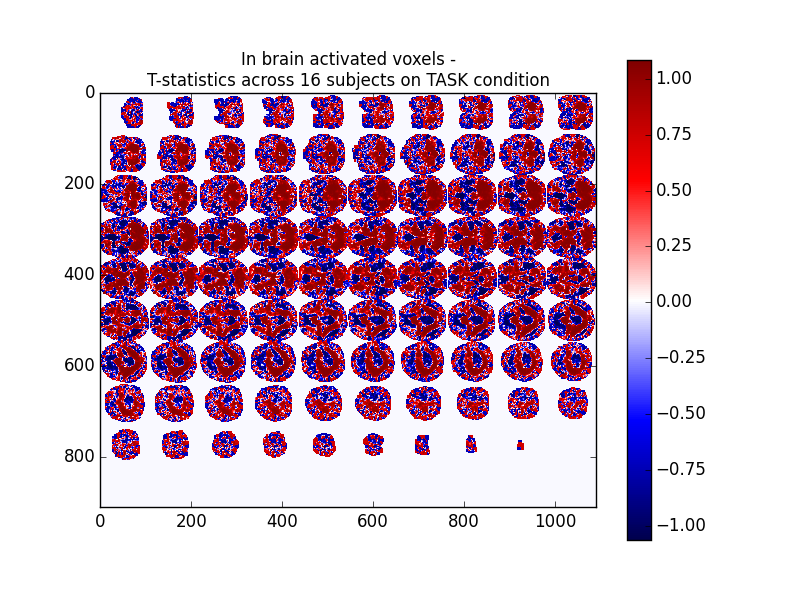
\includegraphics[scale=0.5]{../fig/multi_beta/tstat_task.png}	 
\caption{T-statistics of beta values on each voxel across 16 subjects on TASK condition}
\end{figure} 

\begin{figure}[H] 
\centering 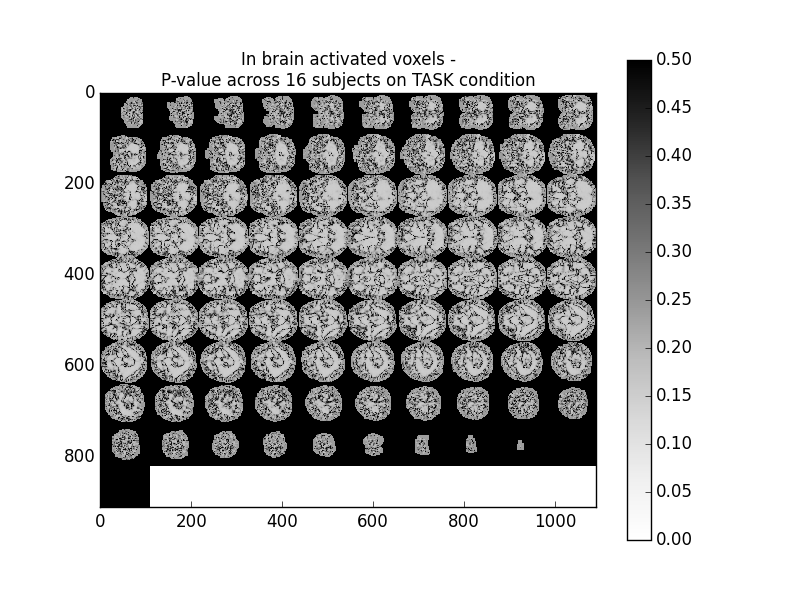
\includegraphics[scale=0.5]{../fig/multi_beta/pval_task.png}	 
\caption{P-value of on each voxel across 16 subjects on TASK condition}
\end{figure} 

\begin{center}
Example 1: Multi-comparison across subjects on TASK condition. P-value indicates the porton of activated
voxels
\end{center}



\subsection{Resource2}

\subsection{Resource3}